%%%%%%%%%%%%%%%%%%%%%%%%%%%%%%%%%%%%%%%%%%%%%%%%%%%%%%%%%%%
%% Congratulations, you've made an excellent choice
%% of writing your Tampere University thesis using
%% the LaTeX system. This document attempts to be
%% as complete a template as possible to let you focus
%% on the most important part: the writing itself.
%% Thus the details regarding the visual appearance
%% and even structure have already been worked out
%% for you!
%%
%% I sincerely hope you will find this template useful
%% in completing your thesis project. I've tried to
%% add comments (followed by the % sign) to clarify
%% the structure and purpose of some of the commands.
%% Most of the magic happens in the file tauthesis.cls,
%% which you are more than welcome to take a look at.
%% Just refrain from editing it in the most crucial
%% versions of the thesis!
%%
%% I wish you and your thesis project the best of luck!
%% If this template causes you trouble along the way
%% or if you've any suggestions for improving it,
%% please contact me via email at
%%
%% ville.koljonen (at) tuni.fi.
%%
%% Yours,
%%
%% Ville Koljonen
%% 16th May 2019
%%
%% PS. This template or its associated class file don't
%% come with a warranty. The content is provided as is,
%% without even the implied promise of fitness to the
%% mentioned purpose. You, as the author of the thesis,
%% are responsible for the entire work, including the
%% provided material. No one else is liable to you for
%% any damage inflicted on you or your thesis, were it
%% caused by using this template or not.
%%%%%%%%%%%%%%%%%%%%%%%%%%%%%%%%%%%%%%%%%%%%%%%%%%%%%%%%%%%

%%%%% NOTICE %%%%%
%% Please read through the entire template
%% (files under ./tex) to find all instructions.
%% It is possible that the attached pdf files
%% do not include the latest information.
%%%%%%%%%%%%%%%%%%

%%%%% INSTRUCTIONS FOR COMPILING THE DOCUMENT %%%%%
%% Overleaf: just click Recompile.
%% Terminal:
%%  1. pdflatex main.tex
%%  2. makeindex main.tex
%%  3. biber main.tex
%%  4. pdflatex main.tex
%%  5. pdflatex main.tex
%% Similar sequence of commands is also required
%% in LaTeX specific editors.
%%%%%%%%%%%%%%%%%%%%%%%%%%%%%%%%%%%%%%%%%%%%%%%%%%%

%%%%% PREAMBLE %%%%%

%%%%% Document class declaration.
% The possible optional arguments are
%   finnish - thesis in Finnish (default)
%   english - thesis in English
%   numeric - citations in numeric style (default)
%   authoryear - citations in author-year style
% Example: \documentclass[english, authoryear]{tauthesis}
%          thesis in English with author-year citations
\documentclass[finnish, authoryear]{config/tauthesis}

% The glossaries package throws a warning:
% No language module detected for 'finnish'.
% You can safely ignore this. All other
% warnings should be taken care of!

%%%%% Your packages.
% Before adding packages, see if they can be found
% in tauthesis.cls already. If you're not sure that
% you need a certain package, don't include it in
% the document! This can dramatically reduce
% compilation time.

% Graphs
\usepackage{pgfplots}
\pgfplotsset{compat=1.15}

% Subfigures and wrapping text
\usepackage{subcaption}

% Mathematics packages
\usepackage{amsmath, amssymb, amsthm}
%\usepackage{bm}

% Chemistry packages
% Newest mhchem is attached for compatibility
\usepackage{chemfig}
\usepackage[version=4]{config/mhchem}

%%%%% Your commands.

% Print verbatim LaTeX commands
\newcommand{\verbcommand}[1]{\texttt{\textbackslash #1}}

% Basic theorems in Finnish and in English.
% Remove [chapter] if you wish a simply
% running enumeration.
\newtheorem{lause}{Lause}[chapter]
\newtheorem{theorem}[lause]{Theorem}

% Use the commented version for individually
% enumerated lemmas
\newtheorem{apulause}[lause]{Apulause}
\newtheorem{lemma}[lause]{Lemma}
% \newtheorem{apulause}{Apulause}[chapter]
% \newtheorem{lemma}{Lemma}[chapter]

% Definition style
\theoremstyle{definition}
\newtheorem{maaritelma}{Määritelmä}[chapter]
\newtheorem{definition}[maaritelma]{Definition}
% examples in this style

%%%%% Glossary information.

\loadglsentries[main]{tex/04_sanasto.tex}
\makeglossaries

%%%%% Citation information.

\addbibresource{tex/00_zotero-referenssit.bib}

\begin{document}

%%%%% FRONT MATTER %%%%%

\frontmatter

%%%%% Thesis information and title page.

% The titles of the work. If there is no subtitle,
% leave the arguments empty. Pass the title in
% the primary language as the first argument
% and its translation to the secondary language
% as the second.
\title{Web-käyttöliittymän hyväksymistestauksen priorisointi painotetun verkon avulla}{Prioritizing Web user interface acceptance testing with a weighted graph}
\subtitle{}{}

% The author name.
\author{Jukka Pajarinen}

% The finishing date of the thesis (YYYY-MM-DD).
\finishdate{2019}{05}{16}

% The type of the thesis (e.g. Kandidaatintyö
% or Master of Science Thesis) in the primary
% and the secondary languages of the thesis.
\thesistype{Opinnäytetyön taso}{Thesis type}

% The faculty and degree programme names in
% the primary and the secondary languages of
% the thesis.
\facultyname{Tiedekunnan nimi}{Faculty Name}
\programmename{Tutkinto-ohjelma}{Degree Programme}

% The keywords to the thesis in the primary and
% the secondary languages of the thesis
\keywords%
    {avainsana, avainsana, avainsana, avainsana, avainsana}
    {keyword, keyword, keyword, keyword, keyword}

\maketitle

%%%%% Abstracts and preface.

% Write the abstract(s) and the preface
% into a separate file for the sake of clarity.
% Pass the appropriate file name as the first
% argument to these commands. Put the \abstract
% in the primary language first and the
% \otherabstract in the secondary language second.
% Those who do not speak Finnish only need the
% first abstract. The second argument of
% the \preface command takes the place where
% the thesis was signed in.
\abstract{tex/01_tiivistelma.tex}
\otherabstract{tex/02_abstract.tex}
\preface{tex/03_alkusanat.tex}{Tampereella}

%%%%% Table of contents.

\tableofcontents

%%%%% Lists of figures, tables, listings and terms.

% Print the lists of figures and/or tables.
% (Un)comment either of these commands as required.
% Both are optional, but if there are many important
% figures/tables, listing them may be a good idea.

%\listoffigures
%\listoftables
%\lstlistoflistings

% Print the glossary of terms.

\glossary

%%%%% MAIN MATTER %%%%%

\mainmatter

% Write each of the chapters of the thesis
% into a separate file for the sake of clarity.
% They can be \input as shown below. Give both
% the chapters and their files as descriptive
% names as possible.
\chapter{Johdanto}
\label{ch:johdanto}
Tämä mallipohja liittyy Tampereen yliopiston tekniikan alan opinnäytteiden kirjoitusohjeisiin \parencite{kirjoitusohje2018}. Opinnäyte koostuu tyypillisesti seuraavista osista:

\begin{enumerate}
    \item[] Nimiölehti
    \item[] Tiivistelmä suomeksi ja englanniksi
    \item[] Alkusanat
    \item[] Sisällysluettelo
    \item[] (Kuva- ja taulukkoluettelot)
    \item[] Lyhenteet ja merkinnät
    \item Johdanto
    \item Teoreettinen tausta, lähtökohdat tai ongelman asettelu
    \item Tutkimusmenetelmät ja aineisto
    \item Tulokset ja niiden tarkastelu (mahdollisesti eri luvuissa)
    \item Yhteenveto ja/tai päätelmät
    \item[] Lähdeluettelo
    \item[] (Liitteet)
\end{enumerate}

Jokainen yllämainituista osista kirjoitetaan omaksi luvukseen (\verbcommand{chapter}) tai asianmukaisella komennolla (esim. \verbcommand{abstract}). Lue pohja ja sen kommentit huolella läpi. Osioiden 1--5 nimet ovat tässä ainoastaan esimerkkejä. Käytä työssäsi paremmin sisältöä kuvaavia nimiä. Nimiölehti luodaan täyttämällä asianmukaiset tiedot komentoihin pohjan alkupuolella. Sisällysluetteloon kootaan kaikki sitä seuraavat otsikot, erityisesti numeroidut. Aina siihen ei laiteta osia ennen sisällysluetteloa.

Johdannossa herätetään lukijan mielenkiinto, perehdytetään hänet tutkimuksen aihepiiriin ja jäsennetään tutkimus. Seuraavaksi esitellään opinnäytetyön taustatiedot, jotka ovat välttämättömiä työn ongelman ymmärtämiselle. Toisinaan tässä kuvataan myös käytetyt menetelmät ja aineisto, eli miten tutkimus on toteutettu.

Sen jälkeen esitellään työssä saavutetut tulokset, niiden merkitys, virhelähteet, poikkeamat oletetuista tuloksista ja tulosten luotettavuus. Yhteenveto on työn tärkein osio. Siinä ei enää toisteta yksityiskohtaisen tarkkoja tuloksia, vaan päätulokset kootaan yhteen ja pohditaan niiden merkitystä. Lähdeluettelo antaa kuvan työn teoreettisesta ja empiirisestä pohjasta sekä toimii kirjallisuusluettelona. Siinä esitetään kaikki tarvittavat tiedot kunkin julkaisun löytämiseksi.

Tämän pohjan luvussa \ref{ch:esitystyyli} käsitellään kuviin, taulukoihin ja matemaattisiin merkintöihin liittyvät esitystyylin perussäännöt. Luvuissa \ref{ch:viittaustekniikat} ja \ref{ch:yhteenveto} esitellään viittaustekniikat ja lyhyt yhteenveto. Jokaisessa kohdassa annetaan lisäksi vinkkejä joidenkin yksityiskohtien ratkaisemiseen \LaTeX{}illa.

\chapter{Tutkimusasetelma}
\label{ch:tutkimusasetelma}
Tässä luvussa esitetään diplomityön tausta, tutkimuskysymykset, käytetty tutkimusmenetelmä, tutkimuksen rajaus sekä tavoitteet.
Tutkimuskysymykset liittyvät vahvasti yhteiseen hyväksymistestauksen testitapauksien priorisoinnin teemaan, johon tässä työssä erityisesti keskitytään.
Tutkimus on soveltavaa ja sen tarkoituksena on muodostaa selvitys tutkimusongelman ratkaisemiseksi.
Tässä työssä se tarkoittaa erityisesti matemaattisen, toistettavissa olevan menetelmän kehittämistä hyväksymistestauksen testitapauksien priorisointiongelman ratkaisemiseksi.
Tutkimuskysymyksistä \ref{ch:06_tutkimuskysymykset} itsessään voi päätellä tutkimuksen tarkoitusta ja tavoitteita, mutta tämä esitetään myös yksityiskohtaisemmin tavoitteet luvussa \ref{ch:06_tavoitteet}.
Yhtenä diplomityön osana on myös toteutuksellinen osuus \ref{ch:08_testausjarjestelma_ja_kayttoonotto}, joka on tehty diplomityön asiakasyrityksen tarpeita varten.
Toteutuksellisessa osuudessa esitetään hyväksymistestausjärjestelmä, joka mahdollistaa tutkimusongelmaan liittyvien priorisoitavien testitapauksien toteuttamisen.

\section{Tausta} \label{ch:06_tausta}

  Diplomityö tehtiin WordDive nimiselle yritykselle. WordDive on vuonna 2009 perustettu, Tampereella toimiva, suomalainen kieltenoppimiseen keskittyvä yritys.
  WordDivellä oli kirjoitushetkellä kieltenoppimissovellus mobiilialustalle sekä web-alustalle.
  Tämän diplomityön sisältö koskettaa vain web-alustalla toimivaa sovellusta.
  Hyväksymistestauksen osalta mobiilisovellukselle oli yrityksessä jo toteutettu testiautomaatio, mutta web-alustalle sitä ei vielä oltu tehty.

  Allekirjoittanut aloitti työt kyseisessä yrityksessä 2018 vuoden loppupuolella, jolloin diplomityön aihetta ei vielä ollut.
  Tarkoituksena oli tuolloin ensin töitä tekemällä tutustua yrityksen web-alustalla toimivaan sovellukseen ja yrityksen ohjelmistotuotantoprosessiin.
  Diplomityön aihe alkoi muotoutua vasta vuoden 2019 alkupuolella, kun tarvittava tietämys ohjelmistotuotteesta ja prosessista oli saavutettu.
  Asiakasyrityksessä sai hyvinkin vapaasti löytää itseään kiinnostavan, varsinaisten töiden ohella tehtävän, mutta kaikille osapuolille hyödyllisen aiheen.
  Aiheen löytämisen taustalla olivat hyvinkin konkreettiset tarpeet, jotka ohjelmistotuotannon työssä tulivat esille.

  Uusien ominaisuuksien ja koodimuutoksien tekemisen yhteydessä oli jatkuvasti tarve huolelliselle testaamiselle ja erityisesti asiakkaan näkökulmasta tärkeimpien sovelluksen ominaisuuksien toiminnan varmistamiselle.
  Tämä sai diplomityön aiheen suuntautumaan testiautomaatioon ja erityisesti hyväksymistestaukseen.
  Lisäksi yrityksessä oli jo toteutettuna päivittäisessä käytössä oleva hyväksymistestaus mobiilialustalle, joka auttoi hahmottamaan web-sovelluksen testiautomaation integroimista osaksi yrityksen ohjelmistotuotantoprosessia.
  Mobiilialustalle tehtyä hyväksymistestausta varten oli yrityksessä jo valittu tietyt hyväksi todetut sovelluskehykset ja työkalut testiautomaatiota varten, joten tässä työssä ei enää ollut tarvetta evaluoida eri työkaluja tarvittavan testiautomaation toteuttamiseksi.
  Web-sovelluksen testiautomaatio toteutettiin käyttäen pääpiirteittäin samoja sovelluskehyksiä ja työkaluja kuin mobiilisovellukselle \ref{ch:08_hyvaksymistestausjarjestelma}.
  Tästä syystä diplomityön aihetta ja tutkimusongelmaa lähdettiin etsimään muualta.

  Tutkimusongelmaan mietittiin aihioita etenkin alkuvaiheessa polkutestauksen ja ohjelmistotestaukseen liittyvien heuristiikkojen osalta.
  Polkutestaus oli yhtenä vaihtoehtona, mutta siitä luovuttiin, koska sen todettiin olevan paremmin soveltuvampi hyväksymistestausta alemmille testauksen tasoille.
  Heuristiikkojen hyödyntämistä mietittiin kahteen eri ongelmaan; testitapauksien muodostamiseen sekä kriittisten testitapauksien määrittämiseen.

  Lopullisen tutkimusongelman löytämiseen vaikuttivat erityisesti konkreettiset tarpeet, jotka tulivat esiin vasta web-sovelluksen testiautomaation suunnitteluvaiheessa.
  Hyväksymistestauksen testiautomaatiota varten oli ensin määritettävä mitä testauksen kohteena olevasta sovelluksesta tulisi testata.
  Testiautomaation rakentamiseen allokoitavia resursseja oli rajallinen määrä, jonka lisäksi testikattavuuden suppeus sekä ylikattavuus nähtiin selkeänä ongelmana.
  Tämä ongelma voidaan esittää yksinkertaisemmin testitapauksien priorisointiongelmana, joka myös lopulta muotoutui työn tutkimusongelmaksi.
  Priorisointiongelman valitsemiseen ratkaisevasti johtavia asioita olivat kaksi allekirjoittaneen oivallusta aiheesta.
  Ensimmäiseksi hyväksymistestattavaa web-sovellusta keksittiin ajatella käyttöliittymän näkymä- ja siirtymätasolla matemaattisena prioriteetein painotettuna verkkona.
  Toiseksi oivallukseksi keksittiin käyttää lyhimmän polun ongelmaan kehitettyjä algoritmeja prioriteetein painotettuun verkkoon, jolloin kahden solmun välille voitiin löytää prioriteeteiltaan korkein polku.
  Nämä oivallukset vaikuttivat lopulta varsinaisen tutkimusongelman eli testitapauksien priorisointiongelman valitsemiseen, koska ne loivat järkevän ja mielenkiintoisen pohjan tutkimusongelmaan vastaamiselle.
  Kokonaisuutena diplomityön aihe saatiin muodostettua sellaiseksi, että se esittää yleishyödyllisen menetelmän tutkimusongelman ratkaisemiseen sekä siihen liittyvän toteutuksen suunnittelemisen ja rakentamisen asiakasyritykselle.

\section{Tutkimuskysymykset} \label{ch:06_tutkimuskysymykset}

  Tutkimuksen tarkoituksena on pohjimmiltaan tarkoitus löytää ja kehittää toistettavissa oleva menetelmä hyväksymistestauksen testitapauksien priorisoimiseen.
  Testitapauksien laatimisen yleisenä ongelmakohtana on erityisesti niiden priorisointi, joka usein johtaa liian suppean tai ylikattavan testiautomaation rakentamiseen.
  Tutkimuskysymykset on laadittu siten, että niihin vastaaminen antaa ratkaisun tähän edellä mainittuun testiautomaation ongelmaan.

  Työlle asetettiin seuraavat tutkimuskysymykset:

  \begin{itemize}
    \item \textbf{T1:} \emph{Miten painotettua verkkoa voidaan käyttää testitapauksien priorisoimiseen?}
    \item \textbf{T2:} \emph{Mitkä muuttujat vaikuttavat web-käyttöliittymän hyväksymistestauksen testitapauksien priorisointiin?}
    \item \textbf{T3:} \emph{Kuinka prioriteetein painotetusta verkosta valitaan toteutettavat testitapaukset?}
    \item \textbf{T4:} \emph{Miten painotetun verkon avulla tehty priorisointi liitetään yhteen jatkuvan integraation ja testiautomaation kanssa?}
  \end{itemize}

  \section{Tutkimusmenetelmä} \label{ch:06_tutkimusmenetelma}

  Tutkimuskysymyksiin vastaamiseksi työn tutkimusmenetelmäksi valittiin tietotekniikan diplomitöissä yleisesti käytetty Design Science -menetelmä.
  Menetelmän tarkoituksena on tuottaa teknologiaa hyödyntävä ratkaisu tutkimusongelmaan vastaamiseen.
  Valittua menetelmää käytettäessä pyritään tutkimaan uusia ratkaisumalleja ratkaisemattomiin ongelmiin tai kehittämään parempia ratkaisumalleja jo aiemmin ratkaistujen ongelmien tilalle.
  Tietotekniikan tutkimuksessa on aikojen saatossa kehitetty uusia tai parempia tietokonearkkitehtuureja, ohjelmointikieliä, algoritmeja, tietorakenteita ja tiedonhallintajärjestelmiä.
  Näiden osalta yhteistä on, että niissä on monesti käytetty usein jopa tiedostamatta Design Science -menetelmää. % TODO: Lähde?

  Tutkimuksen tarkoituksena oli muodostaa uudenlainen ja toistettavissa oleva menetelmä tutkimuksen kohteena olevan ongelman ratkaisemiseksi.
  Tutkimusidean hahmottelemisen ja ratkaisua kaipaavan ongelman identifioinnin jälkeen, valittua tutkimusmenetelmää käyttäen ensin määriteltiin tutkimuskysymykset \ref{ch:06_tutkimuskysymykset}.

  Seuraavaksi kartoitettiin ratkaisuvaihtoehto tutkimuskysymyksiin ja työn yleiseen priorisoinnin teemaan vastaamiseksi ja esitetään perustelut painotettua verkkoa hyödyntävään ratkaisumenetelmään päätymiseen \ref{ch:09_matemaattisten_verkkojen_tarkoitus}.
  Tutkimusta varten kerättiin teoreettista aineistoa, jonka tarkoituksena oli tukea menetelmän kehittämistä ja jonka avulla pyrittiin luomaan lukijalle mahdollisimman vahva teoreettinen pohja tutkimuskysymyksiin vastaavan ratkaisumenetelmän ymmärtämiseksi.
  Asiakasyrityksen ohjelmistotuote ja ohjelmistotuotantoprosessi huomioiden toteutettiin myös testausjärjestelmä, joka mahdollistaa testiautomaation toteuttamisen ja työssä kehitetyn priorisoinnin ratkaisumenetelmän hyödyntämisen.

  Lopuksi vielä evaluoitiin menetelmän eli ratkaisun ja sitä hyödyntävän toteutuksen toimivuus ja esitetään yhteenveto tutkimuksesta.

\section{Tutkimuksen rajaus} \label{ch:06_tutkimuksen_rajaus}

  Ohjelmistotestauksen tasojen osalta tutkimus rajoittuu hyväksymistestaukseen.
  Tämä rajaus pohjautuu ohjelmistotuotannon työssä konkreettisesti havaittuun tarpeeseen sekä yhdenmukaisen testiautomaation toteuttamiseen mobiili- ja web-sovelluksille asiakasyrityksessä.

  Testitapauksien osalta on olemassa lukuisia eri testausalustoja, joita hyödyntäen testitapauksia voidaan toteuttaa.
  Tässä työssä testitapauksien toteuttaminen rajataan tietylle ennalta määräytyneelle hyväksymistestaukseen tarkoitetulle Robot Framework -alustalle.
  Tämä rajaus pohjautuu asiakasyrityksessä jo aiemmin valittuihin testauksen sovelluskehyksiin ja työkaluihin.
  Lisäksi Robot Framework on alustana yleisesti käytetty ja erityisen hyvin soveltuva etenkin hyväksymistestauksen toteuttamiseen.
  Robot Framework on soveltuu myös hyvin sellaisiin tilanteisiin, joissa halutaan ohjelmointikielillä määritettyjä testitapauksia korkeampaa abstraktiotasoa.

  Jatkuvan integroinnin osalta tutkimus rajoittuu perusteisiin ja tutkimuksen painoarvo pidetään testitapauksien toteuttamisessa ja niiden priorisoinnissa.
  Jatkuva integrointi on kuitenkin asiakasyrityksessä tärkeä osa testiautomaation ja jatkuvan käyttöönoton toteutuksessa.
  Jatkuvan integroinnin osalta ei tässä työssä esitetä muuta kuin testiautomaation toteutusosaan kokonaisuutena erityisesti liittyvät käsitteet ja ratkaisu.
  Tämä rajaus pohjautuu tutkimusongelman tarkempaan spesifioimiseen ja tutkimuksen kokonaislaajuuden hallitsemiseen.

  Verkkoteorian osalta tutkimus rajoittuu perusteisiin ja painotettua verkkoa sekä kehitettyä menetelmää tukeviin käsitteisiin.
  Tämä rajaus pohjautuu työn kohdentamiseen ohjelmistotuotantoon ja diplomityön kirjoitusvaiheessa saatuun ohjauspalautteeseen, jossa matematiikan osuus oli kasvanut liiallisen suureksi.

  Priorisointiin vaikuttavien muuttujien osalta tutkimus rajoittuu muuttujien kartoittamiseen, mutta niiden määrittäminen jätetään työn ulkopuolelle.
  Tämä tarkoittaa käytännössä sitä, että jokainen menetelmää hyödyntävä taho hankkii itse varsinaiset numeeriset arvot muuttujille.
  Esimerkiksi liiketoiminnallisen vision numeerinen arvo on yksinomaan menetelmää käyttävän tahon harkittavissa.

  Lyhimmän polun etsimiseen painotetusta verkosta on olemassa lukuisa määrä erilaisia algoritmeja, mutta tässä työssä hyödynnetään vain perinteistä Dijkstran algoritmia.
  Tämä rajaus pohjautuu työssä kehitetyn priorisointimenetelmän käyttämisen perimmäiseen tarkoitukseen, jossa ei algoritmin tehokkuudella tai lisäominaisuuksilla ole suurta merkitystä.
  Lisäksi Dijkstran algoritmi on selkeä, paljon tutkittu ja käytetty ratkaisu lyhimmän polun etsimiseen sekä sitä käytetään tässä työssä vain jo priorisoidussa verkossa tapahtuvaan analysointiin.

\section{Tavoitteet} \label{ch:06_tavoitteet}

  Tutkimuksen primäärisenä tavoitteena oli kehittää toistettavissa oleva matemaattinen menetelmä web-käyttöliittymien hyväksymistestauksessa tarvittavien testitapauksien priorisointiongelman ratkaisemiseksi.
  Kehitetyn menetelmän tavoitteena on tarjota ratkaisua, joka helpottaa ja tehostaa kyseisen hyväksymistestaukseen liittyvän testiautomaation sekä siihen liittyvien testitapauksien suunnittelua ja rakentamista.

  Primääritavoitteen lisäksi valmiin diplomityön tavoitteena on myös tarjota selkeä, eheä ja helposti ymmärrettävä kokonaisuus hyväksymistestauksen testitapauksien priorisoimiseen, työssä kehitettyä menetelmää käyttäen.
  Kehitetty priorisointimenetelmä pyritään esittämään siten, että valmiista diplomityöstä olisi mahdollisimman paljon hyötyä sen käyttämistä harkitseville tai käyttäville tahoille.

  Tutkimusta ja tutkimusmenetelmää itsessään ajatellen tavoitteena oli tarjota ratkaisumalli ja ratkaisut aiemmin esitettyihin tutkimuskysymyksiin \ref{ch:06_tutkimuskysymykset}.
  Lisäksi tutkimusmielessä tavoitteena oli pystyä todentamaan kehitetyn menetelmän toimivuus käytännössä menetelmää itsessään sekä asiakasyritykselle sen lisäksi tehtyä testausjärjestelmän toteutusta evaluoimalla.
  Evaluointi esitetään diplomityön lopussa ja se esitetään erikseen menetelmälle sekä toteutukselle.


\chapter{Testiautomaatio}
\label{ch:testiautomaatio}
Tässä luvussa esitetään perusteet ja tarvittavat tiedot ohjelmistojen testauksesta ja testiautomaatiosta, jotka liittyvät työn laajempaan teoreettiseen kehykseen.
Ensin esitetään testiautomaation tarkoitus, jonka jälkeen käydään yksityiskohtaisesti läpi ohjelmistotestauksen tasot ja pohditaan niiden merkitystä testiautomaatiossa.
Lopuksi vielä esitetään tarvittavia jatkuvan integroinnin ja testausvetoisen kehityksen perusteita sekä pyritään luomaan lukijalle ymmärrystä siitä miten ne liittyvät niitä laajempaan testiautomaation käsitteeseen.
Testiautomaation perusteiden ymmärtämistä tarvitaan varsinkin työn myöhemmässä vaiheessa, jossa esitetään testiautomaatioon liittyvien testitapauksien varsinainen priorisointi painotetun verkon avulla.

\section{Testiautomaation tarkoitus} \label{ch:07_testiautomaation_tarkoitus}

  Testiautomaation tarkoitus on pohjimmiltaan mahdollistaa ohjelmistotuotteen jatkuva, tehokas ja vaivaton laadunvarmistus, nyt ja tulevaisuudessa.
  Testiautomaation vastakohtana voidaan ajatella manuaalista testausta, joka vaatii täydellistä ihmisen interaktiota testauksen suorittamiseen.
  Testiautomaatiossa käytetään erityisiä ohjelmistotyökaluja ennalta määritettyjen testitapauksien suorittamiseen, ihmisen tekemän manuaalisen testauksen sijaan.
  Ohjelmistojen testaamisella itsessään pyritään löytämään ohjelmistotuotteesta virheitä, anomalioita ja varmistamaan, että se toimii asetettujen vaatimusten sekä suunnitelmien mukaisesti.
  Testauksen automatisoiminen vapauttaa aikaa, kustannuksia ja henkilöresursseja manuaalisesta testaamisesta muihin tuotantotehtäviin sekä parantaa toistettavien testien luotettavuutta poistamalla manuaalisessa testauksessa tapahtuvat inhimillisen virheet.
  Testiautomaatiolla, joka kytketään osaksi ohjelmistotuotantoprosessia, voidaan myös löytää ohjelmistokehityksen aikana ohjelmistokoodiin lipsuvia virheitä ja näin ollen saavuttaa mahdollisuus korjata niitä ennen kuin ohjelmisto julkaistaan loppukäyttäjille (UAT).

  Laadunvarmistuksen osalta ohjelmistokehityksessä on usein käytetty niin sanottuja laadullisia ominaisuuksia, joiden kattamisella voidaan validoida laatua.
  Laadullisia ominaisuuksia ovat ISO 9126-standardin mukaan: toiminnallisuus, luotettavuus, käytettävyys, tehokkuus, ylläpidettävyys ja siirrettävyys \parencite{iso_9126-1_2001}.
  Näistä laadullisista ominaisuuksista testiautomaatiolla pystytään kattamaan erityisesti toiminnallisia, luetettavuudellisia ja tehokkuudellisia ominaisuuksia.
  Käytettävyyden, ylläpidettävyyden ja siirrettävyyden validointi puolestaan on vaikeampaa testiautomaation avulla, sillä ne ovat varsin subjektiivisia.
  Tässä diplomityössä testiautomaation yhteydessä keskitytään erityisesti toiminnallisiin laatuominaisuuksiin ja niiden testaamiseen.

\section{Testauksen tasot} \label{ch:07_testauksen_tasot}

  Testauksen tasoja on useita ja usein ohjelmistojen kattavaan testaamiseen on suositeltavaa käyttää ohjelmistotuotantoprosessissa eri tasojen yhdistelmää.
  Ohjelmistojen testaus usein jaotellaan kolmeen erilaiseen menetelmään, jotka myös vaikuttavat eri testauksen tasojen käyttökelpoisuuteen.
  Erilaisia menetelmiä ovat mustalaatikkotestaus, harmaalaatikkotestaus ja valkolaatikkotestaus, jotka eroavat toisistaan yleisesti ottaen siinä, otetaanko tieto ohjelmistotuotteen sisäisestä toteutuksesta mukaan itse testaamiseen.
  Testauksen tasot esitetään kirjallisuudessa usein hieman eri muodoissa, mutta yleisesti ne jaetaan neljään eri tasoon, jotka voidaan kuvata pyramidin tasoavaruuteen projisoituna muotona.

  \begin{figure}[H]
    \centering
    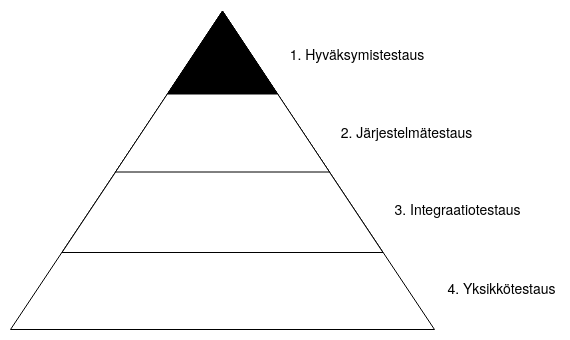
\includegraphics[width=0.8\textwidth]{assets/testauksen-tasot.png}
    \caption{Testauksen tasot pyramidin muodossa}
    \label{fig:testing-levels-pyramid}
  \end{figure}

  Pyramidimuodossa esitetyistä testauksen tasoista kaikkiin on mahdollista soveltaa testiautomaatiota.
  Testauksen menetelmien osalta hieman yksinkertaistaen valkolaatikkotestauksen alaisuuteen kuuluvat yksikkötestaus ja integraatiotestaus sekä mustalaatikkotestauksen alaisuuteen kuuluvat järjestelmätestaus ja hyväksyntätestaus.
  Pyramidimuodossa alimpana kuvataan aina yksikkötestaus, joka on tasoista atomisin ja myös luo vahvan pohjan kokonaisvaltaiselle testaamiselle.
  Noustessa pyramidissa ylöspäin, atomisuus häviää ja testattavana olevan kohteen laajuus sekä kompleksisuus kasvaa.
  Ylimpänä pyramidissa on hyväksymistestaus, joka on tarkoituksellista toteuttaa vaatimusmäärittelyn täyttävää valmista järjestelmää vastaan siten, että sen varmistetaan vastaavan loppukäyttäjän tarpeita.
  Monissa tapauksissa järjestelmätestauksen ja hyväksymistestauksen rajat saattavat olla epäselvät ja häilyvät.
  Tässä työssä hyväksymistestauksella tarkoitetaan käyttäjien hyväksyttämistestausta (UAT), jotta järjestelmätestauksen ja hyväksymistestauksen väliset eroavaisuudet tulevat lukijalle selkeästi esille.

  Hyväksymistestaus on tämän diplomityön keskiössä ja siihen liittyvää teoriaa esitetään vielä laajemmin hyväksymistestaus-luvussa \ref{ch:08_hyvaksymistestaus}.
  Seuraavissa kappaleissa esitetään vielä yksityiskohtaisemmin jokainen pyramidissa \ref{fig:testing-levels-pyramid} esitetty testauksen taso, jotta lukijalle muodostuisi käsitys erityisesti hyväksymistestauksen suhteesta muihin testauksen tasoihin.

  \subsection{Yksikkötestaus} \label{ch:07_yksikkotestaus}

    Yksikkötestauksen ajatuksena on testata ohjelmistotuotteen lähdekoodista löytyviä yksiköitä, kuten luokkia, funktioita tai moduleita.
    Yksikkötestaus toteutetaan ohjelmiston toteuttavia pienimpiä yksikköjä vastaan ja sen avulla pyritään validoimaan, että jokainen yksikkö toimii siten kuin ne on ohjelmistokehityksen aloitusvaiheessa suunniteltu toimimaan.
    Yksikkötestaus eroaa muista testauksen tasoista siinä, että sen voi suorittaa ainoastaan ohjelmistokehittäjät tai muut ohjelmiston lähdekoodiin perehtyneet henkilöt.
    Yksikkötestaus on näin ollen teknisesti valkolaatikkotestausta.
    Yksikkötestausta tarvitaan jotta voidaan pyrkiä varmistamaan, että ohjelmiston pienimmät yksiköt toimivat tarkoituksenmukaisella tavalla.

    Yksikkötestauksen toteuttamiseen käytetään pääsääntöisesti jotakin tarkoitusta varten räätälöityä testikirjastoa, joissa on keskenään yleensä hyvin samankaltainen rakenne.
    Yksikkötestaukseen tarkoitetuissa testikirjastoissa löytyy usein yksittäisen testitapauksen kuvaava tietorakenne, esimerkiksi luokka, sekä siihen usein kuuluvat alustus- ja lopetusfunktiot (setUp ja tearDown).
    Näiden lisäksi varsinainen testauskoodi toteutetaan pääsääntöisesti käyttäen niin sanottuja testikirjaston tarjoamia assert-funktioita, joiden avulla voidaan esimerkiksi varmistaa, onko jokin muuttuja tietyssä arvossa.

    Yksikkötestausta hyödynnetään usein myös ketterien menetelmien aihepiirissä, jossa ohjelmistotuotantoa voidaan toteuttaa muun muassa niin sanotulla testausvetoisella kehityksellä \ref{ch:07_testausvetoinen_kehitys}.
    Testausvetoisessa kehityksessä yksikkötestauksen osalta, ohjelmistokehittäjät laativat ensisijaisesti yksiköiden yksikkötestit ennen niiden toteuttamisen aloittamista.
    Ohjelmistotestauksen tasojen pyramidissa ja hyvin toteutetussa ohjelmistotestauksen monitasoisessa testauksessa tämä testauksen taso on usein kaikista laajin.
    Monitasoisessa testauksessa yksikkötestaus luo tärkeän pohjan testaamiselle kokonaisuutena ja antaa tietoa ohjelmiston pienimpien yksiköiden toimivuudesta.
    Yksikkötestaus on myös paljon käytetty ja tärkeä osa testiautomaatiossa, sillä se varmistaa sovelluksen yksiköiden suunniteltua toimintaa.

  \subsection{Integraatiotestaus} \label{ch:07_integraatiotestaus}

    Integraatiotestauksen ajatuksena on testata ohjelmistotuotteen toteuttavien eri komponenttien yhteentoimivuutta niiden rajapintojen osalta.
    Integraatiotestaus toteutetaan ohjelmiston suunnitelmaa ja mallia vastaan.
    Integraatiotestauksen onnistuminen luo validoitavan perustan ohjelmiston toimimiseen ja sen koostamiseen kokonaisena, eri komponenteista koostuvana järjestelmänä.
    Integraatiotestausta tarvitaan, jotta voidaan varmistaa sovelluksen yksiköiden yhteentoimivuus, joka ei pelkällä yksikkötestauksella tulisi muuten katetuksi.

    Integraatiotestauksen kohteita voivat olla esimerkiksi luokkien ja modulien väliset rajapinnat sekä web-sovelluksien api-ohjelmointirajapinnat.
    Integraatiotestauksen toteutuksen kannalta voidaan usein käyttää myös yksikkötestaukseen tarkoitettuja testikirjastoja ja työkaluja, mutta itse testitapauksien rakenne on silloin merkittävällä tavalla erilainen.
    Integraatiotestauksessa testitapauksien rakenteeseen tulee assert-funktioiden lisäksi myös tarvetta jäljitellä (englanniksi: mocking) rajapintojen tarjoamaa dataa.
    Rajapintojen datan jäljittelemiseen on olemassa useita valmiita työkaluja ja kirjastoja, joita integraatiotestauksen tapauksessa voi käyttää testitapauksien rakentamisen apuna.

    Integraatiotestauksen yhteydessä puhutaan usein myös niin sanotusta savutestauksesta, jonka tarkoituksena integraatiotestauksen yhteydessä on koostaa toistuva, esimerkiksi päivittäinen, koontiversio ohjelmistosta ja testata sen kriittisten komponenttien yhteentoimivuus.
    Integraatiotestaus on myös tärkeä osa testiautomaatiota, sillä sen avulla voidaan varmistaa sovelluksen yksiköiden, kuten esimerkiksi luokkien, komponettien tai modulien yhteentoimivuus.

  \subsection{Järjestelmätestaus} \label{ch:07_jarjestelmatestaus}

    Järjestelmätestauksen ajatuksena on testata kokonaista ja toimivaa järjestelmää, yhtenä suurena yksikkönä.
    Järjestelmätestaus toteutetaan usein eräänlaisena tulikokeena, erityisesti ohjelmiston vaatimuksia vastaan.
    Järjestelmätestausta tarvitaan, jotta voidaan varmistaa kokonaisen ohjelmiston toimivuus, jota ei muuten pelkällä yksikkötestauksella ja integraatiotestauksella saataisi täydellisellä varmuudella selville.
    Järjestelmätestaukseen liittyy laajasti erilaisia testattavia laadullisia ominaisuuksia, kuten toiminnallisuus, luotettavuus, käytettävyys, tehokkuus, ylläpidettävyys ja siirrettävyys \parencite{iso_9126-1_2001}.

    % Järjestelmätestauksen tyyppejä on yli 50, mutta tosiasiassa ohjelmistotestauksessa käytetään vain osaa niistä.
    % Tässä on osittainen lista ohjelmistotuotannossa yleisesti käytetyistä järjestelmätestauksen tyypeistä:

    % \begin{itemize}
    %   \item Regressiotestaus eli toistuva testaus
    %   \item Stressitestaus
    %   \item Toiminnallinen testaus
    %   \item Palautumistestaus
    %   \item Muutostestaus
    %   \item Käytettävyystestaus
    %   \item Alustatestaus
    % \end{itemize}

    <TODO: kirjoita tämä kappale paremmin...>

    Aiemmin testiautomaation tarkoitus kappaleessa \ref{ch:07_testiautomaation_tarkoitus} esitettiin, edellä mainituista laadullisista ominaisuuksista kaikki eivät sovellu hyvin testiautomaation avulla testattaviksi.
    Esitetyistä syistä johtuen, automatisoidulla järjestelmätestauksella voidaan testata edellä mainituista ominaisuuksista lähinnä ohjelmiston toiminnallisuutta, luotettavuutta ja tehokkuutta.
    Sen myötä testauksen tasona se voi olla testiautomaation teknisen toteutuksen kannalta jopa hyvin samanlainen kuin sitä spesifimpi hyväksymistestaus.
    Usein kuitenkin hyväksymistestauksessa paneudutaan erityisesti vaatimusmäärittelyyn ja asiakaslähtöiseen testaamiseen, kun taas järjestelmätestauksessa voidaan testata esimerkiksi myös järjestelmän tehokkuutta tai tietoturvaa.
    Tämä on tosin täysin riippuvainen vaatimusmäärittelystä, ja jos tehokkuus ja tietoturva ovat ohjelmiston asiakasvaatimuksia niin niiltä osin järjestelmätestaus ja hyväksymistestaus lomittuvat.
    Joissakin yhteyksissä järjestelmätestaus ja hyväksymistestaus esitetään jopa yhteisenä testauksen tasona, etenkin silloin kun testiautomaation kannalta ne muistuttavat kovasti toisiaan esimerkiksi edellä mainitulla tavalla.

    Järjestelmätestaus, osittain hyväksymistestauksen kanssa on erittäin merkittävä osa testiautomaatiosta, sillä sen avulla voidaan varmistaa kokonaisen järjestelmän vaadittu toiminnallisuus.

  \subsection{Hyväksymistestaus} \label{ch:07_hyvaksymistestaus}

    Hyväksymistestauksen ajatuksena on varmistaa toteutettavan ohjelmiston vaatimusten toimivuus erityisesti käytännön tilanteissa siten, että voidaan varmistaa vastaako ohjelmisto loppukäyttäjän tarpeita.
    Hyväksymistestaus toteutaan ohjelmiston toimintoja kuvaavaa vaatimusmäärittelyä ja loppukäyttäjistä sekä heidän tarpeista laadittuja käyttötapauksia vastaan.
    Samassa asiayhteydessä puhutaan usein myös niin sanotusta päästä päähän testauksesta (englanniksi: e2e, end-to-end).
    Päästä päähän testauksessa on tarkoituksena toteuttaa testaaminen siten, että polkuina ajateltuna, se sisältää kaiken siltä väliltä mitä loppukäyttäjä voi tarpeidensa saavuttamiseksi tehdä ja nähdä aloittaessaan ohjelmiston käytön ja lopettaessaan sen käytön.
    Testiautomaatio on erittäin hyödyllinen myös hyväksymistestauksen osalla, koska sillä voidaan automatisoida ohjelmiston validointi ja hyväksyminen, sekä estää puutteellisesti toimivan ohjelmiston julkaiseminen.
    Hyväksymistestausta tarvitaan myös, jotta voidaan testata ja validoida vaatimusten mukaisten ominaisuuksien toimivuus.

    <TODO: kirjoita tämä kappale paremmin...>

    Edellisessä kappaleessa käytiin jo hieman läpi järjestelmätestauksen ja hyväksymistestauksen samankaltaisuutta.
    Tässä on asiaa toisinpäin tarkasteltuna, osittainen lista ohjelmistotuotannossa havaittavista järjestelmätestauksen ja hyväksymistestauksen eroista, järjestelmätestauksen näkökulmasta:

    \begin{itemize}
      \item Painoarvo vaatimusmäärittelyssä
      \item Ohjelmistokehittäjien ja testaajien lisäksi myös sidosryhmät ja asiakkaat
      \item Testaus on vain lähinnä toiminnallista
      \item Testauksen syötteet tulevat suoraan käyttäjältä
      \item Testaus keskittyy arvioimaan täyttääkö ohjelmisto käyttäjän tarpeet
      \item A/B testaamisen mahdollisuus
      \item Hyväksymistestaus tapahtuu järjestelmätestauksen jälkeen
      \item Virheet käsitellään epäonnistumisina
    \end{itemize}

    Hyväksymistestaus, osittain järjestelmätestauksen kanssa on äärimmäisen hyödyllinen osa testiautomaatiosta, sillä sen avulla voidaan varmistaa kokonaisen järjestelmän toiminnallisuus ja verifioida, että se vastaa vaatimusmäärittelyä.
    Hyväksymistestauksen rooli testiautomaatiossa ja erityisesti jatkuvan integraation yhteydessä on indikoida voidaanko järjestelmä sellaisenaan julkaista loppukäyttäjille.

\section{Testitapaus ja testikokoelmat} \label{ch:07_testitapaus_ja_testikokoelmat}

  \begin{itemize}
    \item <TODO: Lisää testitapauksen esittely tähän>
    \item <TODO: Lisää testikokoelman esittely tähän>
    \item <TODO: Korosta testikokoelman ja käyttöliittymän näkymän yhteyttä tässä>
  \end{itemize}

\section{Jatkuva integrointi} \label{ch:07_jatkuva_integrointi}

  Testiautomaation rakentaminen manuaalisen testaamisen sijaan mahdollistaa sen liittämisen osaksi jatkuvaa integrointia.
  Lisäksi useissa yritysmaailman ohjelmistotuotannon prosesseissa pelkkä manuaalinen testaus kävisi selkeästi automatisoitujen koonti- tai julkaisuputkien periaatteita vastaan.
  Testiautomaation tarkoitus kappaleessa \ref{ch:07_testiautomaation_tarkoitus} aiemmin esitettiin testiautomaation ja manuaalisen testauksen eroa hyötyjen ja haittojen näkökulmasta.
  Testiautomaation toteuttaminen testitapauksien muodossa on jo itsessään testiautomaatiota, mutta käsitettä voidaan kuitenkin laajentaa, että myös jatkuva integrointi liittyy oleellisesti testiautomaation toteuttamiseen varsinkin nykyaikana ja ketteriin menetelmiin painottuvassa ohjelmistokehityksessä.

  Jatkuvalla integroinnilla tarkoitetaan versiohallintaisessa ohjelmistokehityksessä väistämättömän integrointiprosessin muuntamista jatkuvaksi.
  Ohjelmistokehityksessä integrointiprosessi tulee vastaan, kun eri ohjelmistokehittäjät tai tiimit toteuttavat muutoksia tai uusia ominaisuuksia kehitettävänä olevaan ohjelmistotuotteeseen.
  Tällaisessa tilanteessa yksittäiset ohjelmistokehittäjät tai tiimit toteuttavat uutta ohjelmakoodia toisistaan irrallaan siihen asti kunnes muutokset tai ominaisuudet tulee yhdistää yhdeksi kokonaiseksi kehityksen kohteena olevaksi ohjelmistotuotteeksi, jota prosessina kutsutaan integrointiprosessiksi.
  Jatkuvan integroinnin tarkoituksena on nopeuttaa integrointiprosessia ja muuttaa ohjelmistokehityksessä käytössä olevia periaatteita siten, että siitä tulee luonnostaan jatkuvaa.
  Jatkuvan integroinnin toteuttaminen tarvitsee teknisesti sen mahdollistavan versionhallintajärjestelmän ja varsinaisen jatkuvan integroinnin palvelimen.

  \begin{figure}[H]
    \centering
    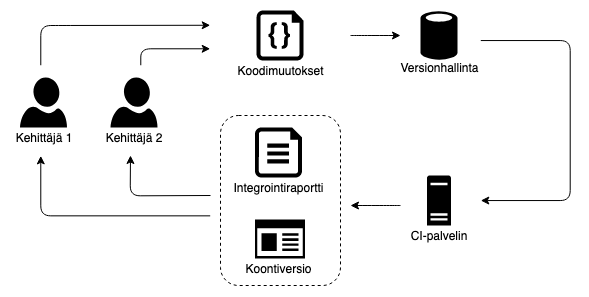
\includegraphics[width=0.8\textwidth]{assets/jatkuva-integrointi.png}
    \caption{Jatkuvan integroinnin perusperiaate on iteratiivinen}
    \label{fig:jatkuva-integrointi}
  \end{figure}

  Esimerkkinä versionhallintajärjestelmänä voidaan käyttää nykyaikana suosittua git versionhallintaohjelmistoa ja jatkuvan integroinnin palvelimena esimerkiksi GoCD ohjelmistoa.
  Perusideana jatkuvassa integraatiossa on konfiguroida jatkuvan integraation mahdollistava ohjelmisto siten, että se kuuntelee versionhallintaan tulevia muutoksia ja suorittaa integrointiprosessin jatkuvasti sellaisia huomattuaan.
  Versionhallintaan tulevat muutokset voidaan jatkuvan integraation osalta kuunnella ajastetusti tietyin väliajoin tai oikeasti jatkuvasti käyttämällä esimerkiksi web-koukkuja, jotka tiedottavat jatkuvan integraation palvelimelle versionhallintaan saapuneista muutoksista.
  Jatkuvan integroinnin yhden iteraatiokerran integrointiprosessin tuloksena on tarkoituksena tarjota periaatteeltaan sama lopputulema kuin mitä se olisi manuaalisella integrointiprosessillakin.
  Jatkuva integroinnin mahdollistava konfiguraatio sisältää jonkinlaisen koontiputken tai koontiputkia, joissa rakennetaan koontiversio kehitettävän ohjelmiston lähdekoodeista.
  Koontiputki voi sisältää esimerkiksi ohjelman lähdekoodien kääntämisen asiaan sopivalla kääntäjällä.
  Kääntämisen lisäksi koontiputkeen on tässä vaiheessa erittäin kannattavaa yhdistää testiautomaatiota, kuten esimerkiksi automaattiset yksikkötestit ennen kääntämistä ja hyväksymistestit kääntämisen jälkeen.

  Jatkuvan integroinnin yhteydessä suoritettavat testikokoelmat ja niiden sisältävät testitapaukset ovat erittäin järkevää toteuttaa, sillä ne esimerkiksi parantavat ohjelmistokehityksen ja lopputuotteen luotettavuutta ja laatua.
  Jatkuvan integroinnin sisältämästä koontiputkesta saadaan hyödyllistä palautetta ja raportteja integrointiprosessin onnistumisesta, joka voidaan ohjata pääasiassa ohjelmistokehittäjille sekä myös muillekin sidosryhmille.
  Jatkuvalla integroinnilla itsessään on myöskin paljon sen käyttöönoton antamia hyötyjä, kuten esimerkiksi toteutettujen muutosten tai toimintojen integrointitiheyden kasvattamisen tuomat edut.
  Jos muutosten tai toimintojen integroiminen on perinteisessä ohjelmistokehitetyksessä tehty esimerkiksi viikoittain, niin jatkuva integroiminen korjaa sen tuomat haasteet turhan laajasta integrointiprosessista ja mahdollisesta ohjelmistokoodin hajoamisesta.
  Tällaisissa tapauksissa ohjelmistokoodi voi sisältää epäyhteensopivia moduleita tai muita rajapintoja sekä mahdollisuuden käännettävien lähdekoodien kääntämisen onnistumisesta.

\section{Testausvetoinen kehitys} \label{ch:07_testausvetoinen_kehitys}

  Perinteisesti testiautomaatio on soveltunut hyvin vain vakaille ohjelmistoille ja niiden regressiotestaamiseen.
  Nykypäivänä ohjelmistokehitys on siirtynyt suunnitelmapohjaisista prosesseista iteroiviin ketteriin ohjelmistotuotannon prosesseihin.
  Näihin testiautomaatio on soveltunut huonosti, kun testattavaa ohjelmistoa tai lisättyä toiminnallisuutta ei ole vielä olemassa.
  Tähän ongelmaan on kehittynyt niin sanottu testausvetoinen kehitys, jossa testitapaukset suunnitellaan ja toteutetaan ennen varsinaisen ohjelmiston tai toiminnon toteutuksen toteuttamista.

  \begin{figure}[H]
    \centering
    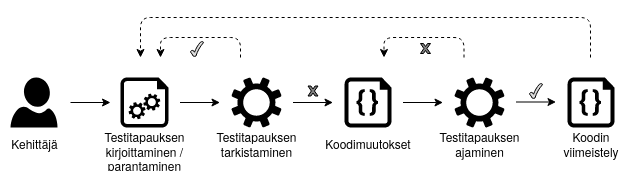
\includegraphics[width=0.8\textwidth]{assets/testausvetoinen-kehitys.png}
    \caption{Testausvetoisen kehityksen vaiheet}
    \label{fig:testausvetoinen-kehitys}
  \end{figure}

  Testausvetoinen kehityksen sisältämät vaiheet \ref{fig:testausvetoinen-kehitys} alkavat testitapauksien luomisesta ja niiden tarkastamisesta.
  Tarkastaminen tapahtuu siten, että testitapaukset ajetaan oletuksella, että niiden täytyy tässä vaiheessa epäonnistua.
  Alkuvaiheen testitapauksien luomisen jälkeen ohjelmistkehittäjät kehittävät ohjelmistoa tekemällä siihen muutoksia ihanteellisesti testitapauksien kokoisia paloja kerrallaan.
  Kun koodimuutoksia on syntynyt, riippuen ohjelmistotuotannossa käytössä olevasta integrointiprosessista, ajetaan testitapaukset manuaalisesti tai jatkuvan integroinnin avulla.
  Integrointiprosessista saadaan palautetta, jonka mukaan ohjelmakoodia korjataan tai viimeistellään.
  Testausvetoisella kehityksellä pyritään nopeuttamaan ohjelmistokehitysprosessia verrattuna perinteisiin ohjelmisttuotannon menetelmiin.
  Tämän jälkeen testausvetoista kehitystä käyttävässä ohjelmistotuotantoprosessissa siirrytään takaisin testitapauksien luomiseen ja parantamiseen sekä aloitetaan toinen iteraatiokierros mikäli ohjelmisto ei vielä ole valmis.

  Testausvetoisessa kehityksessä testitapaukset siis laaditaan jo varhaisessa vaiheessa jolloin niiden tekeminen saattaa usein olla liiketoiminnan näkökulmasta helpommin perusteltavaa liiketoiminnan johdolle.
  Tämän lisäksi testitapauksien kirjoittaminen etukäteen luo kattavat testikokoelmat jo alusta alkaen, joita voidaan hyödyntää iteratiivisesti ohjelmistotuotteesta riippuen usein hyvinkin pitkään, etenkin jos niihin tehdään tarvittavaa hienosäätöä ohjelmistokehityksen aikana.
  Ohjelmistokehittäjät voivat kehittää helposti hallittavissa olevia testitapauksien rajaavia kokonaisuuksia, jolloin ohjelmistotuote valmistuu ikään kuin pala kerrallaan.
  Itse ohjelmistkehitys on siis iteratiivista ja näin ollen testitapauksien suorittamisesta saadaan palautetta ja raportointia koko ohjelmistotuotantoprosessin aikana.
  Testausvetoinen kehitys kuuluu ohjelmistotuotannossa vahvasti ketterien menetelmien alaisuuteen ja on kasvattanut suosiotaan ketterien menetelmien mukana.


\chapter{Jatkuva integraatio}
\label{ch:jatkuva_integraatio}
<Lisää teksti tähän>

\section{Jatkuvan integraatio tarkoitus}

<Lisää teksti tähän>

\section{Jatkuvan integraatio julkaisuputki}

<Lisää teksti tähän>

\section{Muutosperustainen tai ajastettu koostaminen}

<Lisää teksti tähän>

\section{Jatkuvan integraation ja testiautomaation yhdistäminen}

<Lisää teksti tähän>

\section{Hyväksymistestausvetoinen kehitys}

<Lisää teksti tähän>


\chapter{Testitapauksien priorisointi}
\label{ch:testitapauksien_priorisointi}
Tässä luvussa esitetään tutkimuksen tärkein sisältö, eli toistettavissa oleva menetelmä testitapauksien priorisoimiseen.
Priorisointia varten esitetään harkintaa käyttäen lähdeaineistosta suodatetut priorisointiin vaikuttavat muuttujat, painofunktio, testitapauksien näkymäperusteinen koostaminen ja painotetun verkon laatiminen.
Lisäksi menetelmää käyttäen tuotetun painotetun verkon sisältämää informaatiota käytetään prioriteeteiltaan tärkeiden polkujen löytämiseen ja testikattavuuden arviointiin.

\section{Priorisointiin vaikuttavat muuttujat}

\begin{itemize}
  \item Liiketoiminnallinen arvo
  \item Projektin muuttumisen volatiliteetti
  \item Kehittämisen kompleksisuus
  \item Vaatimusten taipumus virheellisyyteen
\end{itemize}

\section{Painofunktio priorisointiin}

\[f(a,b,c,d) = a+b+c+d\]

\section{Testitapauksien koostaminen näkymistä}

<Lisää teksti tähän>

\section{Painotetun verkon rakentaminen}

<Lisää teksti tähän>

\section{Painotetun verkon karsiminen}

<Lisää teksti tähän>

\section{Korkeiden prioriteettien polut}

<Lisää teksti tähän>

\section{Testikattavuuden arviointi}

<Lisää teksti tähän>


\chapter{Testauksen suunnittelu ja toteutus}
\label{ch:testauksen_suunnittelu_ja_toteutus}
Tässä luvussa esitetään työn perusteella tehty esimerkkitoteutus sekä käytännön sovelluskehyksen ja työkalut.
Tämän luvun tarkoituksena on todistaa menetelmän toimivuus oikeassa ohjelmistotuotannon ympäristössä toteuttaen samalla testiautomaatio asiakasyritykselle.

\section{Sovelluskehykset ja työkalut}

<Lisää teksti tähän>

  \subsection{Docker}

  <Lisää teksti tähän>

  \subsection{GoCD}

  <Lisää teksti tähän>

  \subsection{Robot Framework}

  <Lisää teksti tähän>

  \subsection{Selenium}

  <Lisää teksti tähän>

\section{Jatkuva integraatio ja testiautomaatio}

<Lisää teksti tähän>

\section{Painotetun verkon käyttö priorisoimiseen}

<Lisää teksti tähän>

\section{Testitapauksien toteuttaminen}

<Lisää teksti tähän>

\section{Testiautomaation seuranta}

<Lisää teksti tähän>


\chapter{Yhteenveto}
\label{ch:yhteenveto}
<TODO: diplomityön tavoite saavutettu....>

<TODO: tavoitteena oli xxxxxx ....>

<TODO: tutkimuskysymykseen T1 vastattiin luvussa X .....>

<TODO: tutkimuskysymykseen T2 vastattiin luvussa X .....>

<TODO: tutkimuskysymykseen T3 vastattiin luvussa X .....>

<TODO: tutkimuskysymykseen T4 vastattiin luvussa X .....>

<TODO: konkreettisista tuloksista hyötyä......>

<TODO: diplomityö loi perustan asiakasyrityksessä tarvittavan testiautomaation rakentamiseen...>

%%%%% Bibliography/references.

% Print the bibliography according to the
% information in ./tex/references.bib and
% the in-line citations used in the body of
% the thesis.
% \emergencystretch=2em
\printbibliography[heading=bibintoc]

%%%%% Appendices.

% Use only if it clarifies the structure of
% the document. Remember to introduce each
% appendix and its content.

\begin{appendices}

\chapter{Esimerkkiliite}
\label{ch:liite}
<Lisää teksti tähän>

\end{appendices}

\end{document}